\section{Rule Count at a Fixed Long Length (\expE)}
\label{app:expE}

\begin{figure}[h]
    \centering
    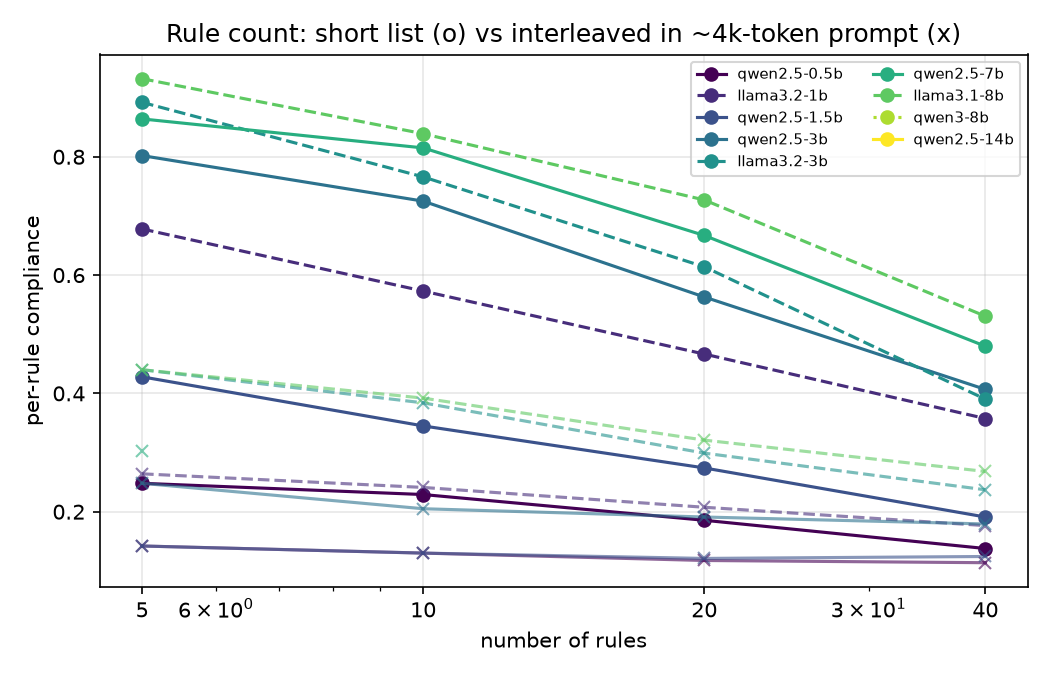
\includegraphics[width=0.62\linewidth]{figures/expE_count_long.png}
    \caption{\expE: per-rule compliance as the number of rules grows, with all rules interleaved in about 4k tokens of padding, compared with the short numbered-list format of \expA. Compliance still declines with rule count when length is held fixed, but from a much lower starting point.}
    \label{fig:expE}
\end{figure}

\begin{table}[h]
    \centering
    \caption{Per-rule compliance by rule count in a short numbered list (\expA) and interleaved in $\sim$4k tokens of padding (\expE; the $N{=}5$ column is from \expB at 4k tokens). \qseven did not run \expE.}
    \label{tab:expE}
    \small
    \begin{tabular}{@{}lcccccccc@{}}
        \toprule
        & \multicolumn{4}{c}{\textbf{Short list (\expA)}} & \multicolumn{4}{c}{\textbf{Interleaved, $\sim$4k tokens}} \\
        \cmidrule(lr){2-5} \cmidrule(lr){6-9}
        \textbf{Model} & 5 & 10 & 20 & 40 & 5 & 10 & 20 & 40 \\
        \midrule
        \qhalf    & .25 & .23 & .19 & .14 & .14 & .13 & .12 & .11 \\
        \lone     & .68 & .57 & .47 & .36 & .26 & .24 & .21 & .18 \\
        \qonefive & .43 & .35 & .27 & .19 & .14 & .13 & .12 & .12 \\
        \qthree   & .80 & .73 & .56 & .41 & .25 & .21 & .19 & .18 \\
        \lthree   & .89 & .77 & .61 & .39 & \textbf{.44} & .38 & .30 & .24 \\
        \leight   & \textbf{.93} & \textbf{.84} & \textbf{.73} & \textbf{.53} & \textbf{.44} & \textbf{.39} & \textbf{.32} & \textbf{.27} \\
        \bottomrule
    \end{tabular}
\end{table}

\section{Conflict Resolution Details}
\label{app:conflict}

\begin{table}[h]
    \centering
    \caption{\expD: share of responses that satisfy only rule X, only rule Y, or neither, when both contradictory rules are present (``both'' is impossible). X is the first-listed rule of each pair: $<$80 words, concise, bulleted list, lowercase. Largest share per model and pair in \textbf{bold}.}
    \label{tab:winner}
    \resizebox{\textwidth}{!}{%
    \begin{tabular}{@{}lcccccccccccc@{}}
        \toprule
        & \multicolumn{3}{c}{\textsc{length\_hard}} & \multicolumn{3}{c}{\textsc{length\_soft}} & \multicolumn{3}{c}{\textsc{lists}} & \multicolumn{3}{c}{\textsc{case}} \\
        \cmidrule(lr){2-4} \cmidrule(lr){5-7} \cmidrule(lr){8-10} \cmidrule(lr){11-13}
        \textbf{Model} & X & Y & neither & X & Y & neither & X & Y & neither & X & Y & neither \\
        \midrule
        \qhalf     & .12 & .24 & \textbf{.64} & .37 & \textbf{.46} & .17 & \textbf{.58} & .29 & .13 & .32 & \textbf{.38} & .30 \\
        \lone      & .05 & .05 & \textbf{.90} & .01 & \textbf{.90} & .09 & \textbf{.60} & .38 & .02 & .15 & \textbf{.67} & .18 \\
        \qonefive  & .00 & .28 & \textbf{.72} & .10 & \textbf{.69} & .21 & .36 & \textbf{.56} & .08 & \textbf{.49} & .44 & .07 \\
        \qthree    & .38 & .04 & \textbf{.58} & .29 & \textbf{.41} & .30 & \textbf{.57} & .39 & .04 & \textbf{.64} & .30 & .06 \\
        \lthree    & .01 & .19 & \textbf{.80} & .01 & \textbf{.85} & .14 & \textbf{.57} & .38 & .05 & \textbf{.53} & .43 & .04 \\
        \qseven    & .16 & .01 & \textbf{.83} & .14 & \textbf{.44} & .42 & \textbf{.63} & .34 & .03 & \textbf{.51} & .37 & .12 \\
        \leight    & .23 & .15 & \textbf{.62} & .02 & \textbf{.78} & .20 & \textbf{.92} & .04 & .04 & \textbf{.63} & .24 & .13 \\
        \qwenthree & .13 & .27 & \textbf{.60} & .10 & \textbf{.49} & .41 & \textbf{.62} & .37 & .01 & \textbf{.64} & .32 & .04 \\
        \qfourteen & .01 & .10 & \textbf{.89} & .04 & \textbf{.69} & .27 & \textbf{.56} & .44 & .00 & \textbf{.51} & .38 & .11 \\
        \bottomrule
    \end{tabular}}
\end{table}

\begin{table}[h]
    \centering
    \caption{\expD: median response length (words) for the length pairs with only rule X, only rule Y, or both rules, and with no rules ($N{=}0$). With both rules, responses settle between the two targets.}
    \label{tab:wordcounts}
    \small
    \begin{tabular}{@{}lccccccc@{}}
        \toprule
        & \multicolumn{3}{c}{\textsc{length\_hard}} & \multicolumn{3}{c}{\textsc{length\_soft}} & \\
        \cmidrule(lr){2-4} \cmidrule(lr){5-7}
        \textbf{Model} & $<$80 & both & $\ge$300 & concise & both & thorough & no rules \\
        \midrule
        \qhalf     & 81.5 & 138.0 & 300.5 & 83.0 & 227.0 & 260.0 & 193.5 \\
        \lone      & 74.0 & 153.0 & 472.5 & 192.0 & 336.0 & 487.5 & 375.5 \\
        \qonefive  & 90.5 & 204.5 & 399.0 & 103.0 & 291.0 & 361.0 & 191.5 \\
        \qthree    & 46.0 & 96.0 & 423.5 & 95.5 & 200.0 & 434.5 & 333.0 \\
        \lthree    & 74.0 & 219.5 & 453.5 & 199.5 & 319.5 & 427.0 & 321.5 \\
        \qseven    & 51.0 & 103.0 & 456.0 & 103.0 & 234.0 & 436.0 & 312.0 \\
        \leight    & 76.0 & 102.0 & 496.0 & 183.0 & 320.5 & 473.0 & 350.5 \\
        \qwenthree & 56.0 & 158.0 & 354.0 & 87.5 & 241.5 & 437.5 & 392.0 \\
        \qfourteen & 67.5 & 164.0 & 434.5 & 139.5 & 295.0 & 401.5 & 342.0 \\
        \bottomrule
    \end{tabular}
\end{table}

\section{Prompt Templates}
\label{app:templates}

In \expA, the system prompt reads ``You are a helpful assistant. Follow these rules in every response:'' followed by the rules as a numbered list.
In \expB and \expE, the prompt opens with: ``You are a helpful assistant. The reference material below is provided for background only. Rules for your responses are marked `Response rule:' and appear throughout this prompt; follow all of them.''
Each rule is then inserted as a standalone paragraph beginning with ``Response rule:'' at a random paragraph boundary of the padding, which is introduced as ``Reference material (background only):''.
In \expF, the five rules form one numbered block placed before, inside, or after the padding.
All prompts are built with seed 42; rule subsets, rule order, and padding paragraphs are drawn independently for each item.
